% !TEX root = ./Vorlesungsmitschrift AGLA 2.tex  
\lecture{Di 28.04. 10:15}{}
\section{Affine Koordinaten}
Koordinaten in einem \( K \)-Vektorraum \( V \). Sei \( \dim V=n \) und \( v_1,\dotsc , v_n \) eine Basis von \( V \). Dann ist die Abbildung
\begin{align*}
    \phi\maps  \begin{aligned}[t]
        K^n&\to V\\
        (x_1,\dotsc,x_n)&\mapsto \sum\limits_{i=1}^{n}x_i v_i
    \end{aligned}
\end{align*}
ein Isomorphismus von \( K \)-Vektorräumen. Jeder Punkt \( \underrelate{\ni}{V}{v}=\sum_{i=1}^{n}x_i v_i \) ist eindeutig bestimmt durch seine \enquote{Koordinaten}
\begin{align*}
    \inf{\phi}(v)=(x_1,\dotsc,x_n)\in K^n.
\end{align*}
\begin{frage*}
    Sei \( X \) ein affiner Raum über einem Körper \( K \). Können wir auch hier die Lage eines Punkte \( p\in X \) durch Angabe von \enquote{Koordinaten} bezüglich einer \enquote{Basis} beschreibe?
    \begin{figure}[H]
        \centering
        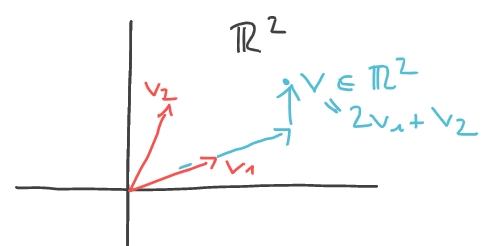
\includegraphics[width=0.5\linewidth]{figures/affine_koordinaten_r_2_hoffnung}
        \label{fig:affine_koordinaten_r_2_hoffnung}
    \end{figure}
    
\end{frage*}
\begin{bspidee*}
    \( X=\reals^2 \) als affiner Raum und Punkte \( p_1,p_2\in X \), sodass \( \vv{p_0p_1} \), \( \vv{p_0p_2} \) eine Basis ist für \( T(X) \). Dann können wir einen Punkt \( p\in X \) beschreiben durch
    \begin{align*}
        p \begin{aligned}[t]
            &=\tau_{\vv{p_0p}}(p_0)\\
            &=\tau_{\lambda\vv{p_0p_1}+\mu\vv{p_0p_2}}(p_0),
        \end{aligned}
    \end{align*}
    falls \( \vv{p_0p}=\lambda\vv{p_0p_1}+\mu\vv{p_0p_2} \) mit \( \lambda,\mu\in \reals \).

    \begin{figure}[H]
        \centering
        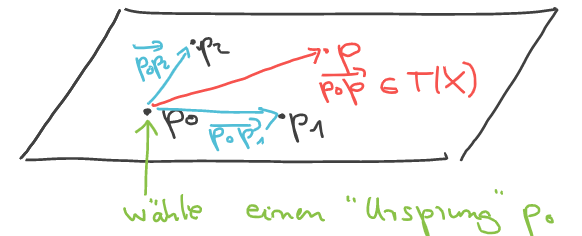
\includegraphics[width=0.5\linewidth]{figures/ursprungswahl}
        \label{fig:ursprungswahl}
    \end{figure}
    
    Wir erhalten eine Abbildung 
    \begin{align*}
        \phi\maps \begin{aligned}[t]
            \reals^2&\to X\\
            (\lambda,\mu)&\mapsto \tau_{\lambda\vv{p_0 p_1}+\mu\vv{p_0 p_2}}(p_0),
        \end{aligned}
    \end{align*}
    die eine Affinität ist.
\end{bspidee*}
Wir formalisieren diese Konzepte für allgemeine affine Räume.
\begin{definition*}
    Sei \( X \) ein affiner Raum und \( p_0,\dotsc, p_n\in X \). Wir nennen \( (p_0,\dotsc,p_n) \) \emph{affin unabhängig} \bzw eine \emph{affine Basis}, wenn die Vektoren \( (\vv{p_0p_1},\dotsc, \vv{p_0p_n}) \) in \( T(x) \) \emph{linear unabhängig sind} \bzw \emph{eine Basis bilden}.
\end{definition*}
\begin{beispiele*}
    \begin{enumerate}
        \item In \( X=\reals^n \) ist \( (0,e_1,\dotsc, e_n) \) eine affine Basis.
        \item \( X=\reals^n \) als affiner Raum, \( v_1,\dotsc, v_k\in \reals^n \) linear unabhängig, \( v_0=0 \). Dann ist das Tupel \( (v_0,v_1,\dotsc,v_k) \) affin unabhängig.
        \begin{frage*}
            Kann man hier \( v_0\in \reals^n \) beliebig nehmen?
        \end{frage*}
        \item \( X=\reals^2 \) als affiner Raum. Dann gilt, dass für \( v,w\in \reals^2 \) das Tupel \( (v,w) \) affin unabhängig ist \gdw \( v\neq w \).
        \item \( X \) affiner Raum, \( p_0\in X \), \( (t_1,\dotsc,t_n) \) Basis von \( T(X) \). Dann ist
        \begin{align*}
            (p_0,\tau_{t_1}(p_0),\dotsc, \tau_{t_n}(p_0))
        \end{align*}
        eine affine Basis von \( X \).
    \end{enumerate}
    
\end{beispiele*}
\begin{lemma}
    Sei \( X \) ein affiner Raum, \( p_0,\dotsc, p_n\in X \) und \( (p_0,\dotsc, p_n) \) affin unabhängig. Sei \( \sigma\in S_{n+1} \) eine Permutation von \( \Set{0,\dotsc,n} \). Dann ist
    \begin{align*}
        (p_{\sigma(0)},p_{\sigma(1)},\dotsc,p_{\sigma(n)})
    \end{align*}
    affin unabhängig.
\end{lemma}
\begin{proof}
    Wir wollen zeigen, dass unter den Annahmen des Lemmas, die Vektoren
    \begin{align*}
        \vv{p_{\sigma(0)}p_{\sigma(1)}},\dotsc,\vv{p_{\sigma(0)p_{\sigma(n)}}}\in T(X)
    \end{align*}
    linear unabhängig sind.

    Sei \( \sigma(0)=i\in \Set{0,\dotsc,n} \).

    Dann müssen wir also zeigen, dass die Vektoren
    \begin{align*}
        \vv{p_i p_0},\vv{p_i p_1},\dotsc, \vv{p_i p_{i-1}},\vv{p_i p_{i+1}},\dotsc,\vv{p_i p_n}
    \end{align*}
    linear unabhängig sind.

    Seien \( \lambda_0,\dotsc, \lambda_{i-1},\lambda_{i+1},\dotsc,\lambda_n\in K \) mit
    \begin{align*}
        \lambda_0 \vv{p_i p_0}+\lambda_1\vv{p_i p_1}+\dotsb+\lambda_{i-1}\vv{p_i p_{i-1}}+\lambda_{i+1}\vv{p_i p_{i+1}}+\dotsb+\lambda_n\vv{p_i p_n}=0.
    \end{align*}
    Schreibe
    \begin{align*}
        \vv{p_i p_j}=\vv{p_i p_0}+\vv{p_0 p_j}=\textcolor{Goldenrod}{\vv{p_0 p_j}}-\textcolor{LimeGreen}{\vv{p_0 p_i}}.
    \end{align*}
    Wir erhalten
    \begin{align*}
        \begin{aligned}[t]
            \textcolor{Goldenrod}{\lambda_1\vv{p_0 p_1}+\dotsb+\lambda_{i-1} \vv{p_0 p_{i-1}}+\lambda_{i+1} \vv{p_0 p_{i+1}}+\dotsb+\lambda_n \vv{p_0 p_n}}\\
            -\textcolor{LimeGreen}{(\lambda_0+\dotsb+\lambda_{i-1}+\lambda_{i+1}+\dotsb+\lambda_n)\vv{p_0 p_i}}=0
        \end{aligned}
    \end{align*}
    Aus der linearen Unabhängigkeit von \( \vv{p_0 p_1},\dotsc, \vv{p_0 p_n} \) folgt
    \begin{align*}
        \lambda_1=\dotsb=\lambda_{i-1}=\lambda_{i+1}=\lambda_n=0
    \end{align*}
    und
    \begin{align*}
            \explain{\lambda_0=0}+\underbrace{\lambda_1+\dotsb+\lambda_{i-1}+\lambda_{i+1}+\dotsb+\lambda_n}_{=0}=0
    \end{align*}
\end{proof}
\subsection*{Affine Basen und affine Abbildungen}
Aus der AGLA \Romannum{1}:\\
Seien \( V,W \) \( K \)-Vektorräume, \( v_1,\dotsc, v_n \in V \) eine Basis von \( V \) und \( w_1,\dotsc, w_n \in W\). Dann gibt es genau eine \( K \)-lineare Abbildung \( \phi\maps V\to W \) mit
\begin{align*}
    \phi(v_i)=w_i,\quad 1\leq i \leq n.
\end{align*}
\begin{figure}[H]
    \centering
    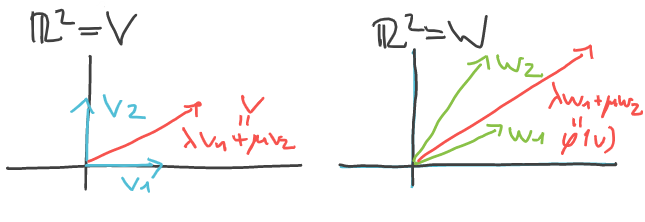
\includegraphics[width=0.7\linewidth]{figures/bilder_der_basen_bestimmt_abbildung_r_2}
    \label{fig:bilder_der_basen_bestimmt_abbildung_r_2}
\end{figure}
\begin{frage*}
    Inwiefern sind affine Abbildungen zwischen affinen Räumen durch die Bilder einer affinen Basis bestimmt?
\end{frage*}
\begin{satz}\label{bilder_der_basen_bestimmen_affine_abbildung}
    Seien \( X,Y \) affine Räume, \( (p_0,\dotsc,p_n) \) eine affine Basis von \( X \) und \( q_0,\dotsc, q_n\in Y \). Dann gibt es genau eine affine Abbildung \( f\maps X\to Y \) mit
    \begin{align*}
        f(p_i)=q_i,\quad 0\leq i\leq n.
    \end{align*}
    Die Abbildung \( f \) ist \emph{injektiv} \bzw \emph{eine Affinität} \gdw das Tupel \( (q_0,\dotsc, q_n) \) \emph{affin unabhängig} \bzw \emph{eine affine Basis} von \( Y \) ist.
\end{satz}
\begin{proof}
    Eine affine Abbildung \( f\maps X\to Y \) ist gegeben durch \( f(p_0) \) für ein \( p_0\in X \) und eine lineare Abbildung
    \begin{align*}
        F\maps \begin{aligned}[t]
            T(X)&\to T(Y)\\
            \vv{pq}&\mapsto \vv{f(p)f(q)}.
        \end{aligned}
    \end{align*}
    Wir definieren \( F \) durch
    \begin{align*}
        F(\vv{p_0 p_i})=\vv{q_0 q_i}\quad 1\leq i \leq n. \tag{*}\label{bilder_der_basen_bestimmt_affine_abbildung:beweis:k_lineare_abbildung}
    \end{align*}
    \( \vv{p_0 p_1}, \dotsc, \vv{p_0 p_n} \) ist eine Basis von \( T(X) \), also gibt es genau ein lineare Abbildung
    \begin{align*}
        F\maps T(X)\to T(Y)
    \end{align*}
    mit \eqref{bilder_der_basen_bestimmt_affine_abbildung:beweis:k_lineare_abbildung}. Es gilt dann
    \begin{align*}
        f(p_i)\begin{aligned}[t]
            &=\tau_{\vv{f(p_0) f(p_i)}} f(p_0)\\
            &=\tau_{F(\vv{p_0 p_i})} f(p_0)\\
            &=\tau_{\vv{q_0 q_i}} q_0 =q_i \quad 1\leq i \leq n.
        \end{aligned}
    \end{align*}
    \( f \) ist injektiv \gdw \( F \) injektiv ist. \( F \) ist injektiv \gdw \( \vv{q_0 q_1}, \dotsc, \vv{q_0 q_n} \) linear unabhängig sind.

    \tto \( f \) ist eine Affinität \gdw \( F \) bijektiv ist. \( F \) ist bijektiv \gdw \( \vv{q_0 q_1}, \dotsc, \vv{q_0 q_n} \) eine Basis von \( T(Y) \) ist.

\end{proof}
\subsection*{Affine Koordinatensysteme}
Sei \( X \) ein affiner Raum über einem Körper \( K \), \( (p_0,p_1,\dotsc, p_n) \) eine affine Basis von \( X \).

Nach \thref{bilder_der_basen_bestimmen_affine_abbildung} gibt es genau eine Affinität
\begin{align*}
    \phi\maps K^n\to X
\end{align*}
mit \( \phi(0)=p_0, \phi(e_1)=p_1,\dotsc, \phi(e_n)=p_n \) und zugehörige lineare Abbildung \( \Phi\maps K^n \to T(X) \).

Einen Punkt \( p\in X \) können wir dann beschreiben durch
\begin{align*}
    p=\tau_{\vv{p_0 p}}(p_0).
\end{align*}
Sei \( \vv{p_0 p}=\lambda_1 \vv{p_0 p_1}+\dotsb +\lambda_n \vv{p_0 p_n} \) mit \( \lambda_i\in K \), \( 1\leq i \leq n \).

Dann ist
\begin{align*}
    p \begin{aligned}[t]
        &=\tau_{\lambda_1\vv{p_0 p_1}+\dotsb +\lambda_n\vv{p_0 p_n}}(p_0)\\
        &=\tau_{\lambda_1 \Phi(e_1)+\dotsb+\lambda_n \Phi(e_n)}(p_0)\\
        &=\tau_{\Phi(\lambda_1 e_1+\dotsb+\lambda_n e_n)}(p_0),
    \end{aligned}
\end{align*}
oder \( p=\phi((\lambda_1,\dotsc,\lambda_n)) \).

\begin{definition*}
    Sei \( X \) ein affiner Raum über einem Körper \( K \). Wir nennen eine Affinität \( \phi\maps K^n\to X \) ein affines Koordinatensystem in \( X \). Seu \( p_0=\phi(0),p_1=\phi(e_1),\dotsc, p_n=\phi(e_n) \). Dann ist \( (p_0,\dotsc,p_n) \) eine affine Basis von \( X \).

    Für \( p\in X \) nennen wir
    \begin{align*}
        \inv{\phi}(p)=(x_1,\dotsc,x_n)\in K^n
    \end{align*}
    den Koordinatenvektor von \( p \) bezüglich der affinen Basis \( (p_0,\dotsc,p_n) \) und \( (x_1,\dotsc, x_n) \) die Koordinaten von \( p \) bezüglich \( (p_0,\dotsc, p_n) \).
    \begin{figure}[H]
        \centering
        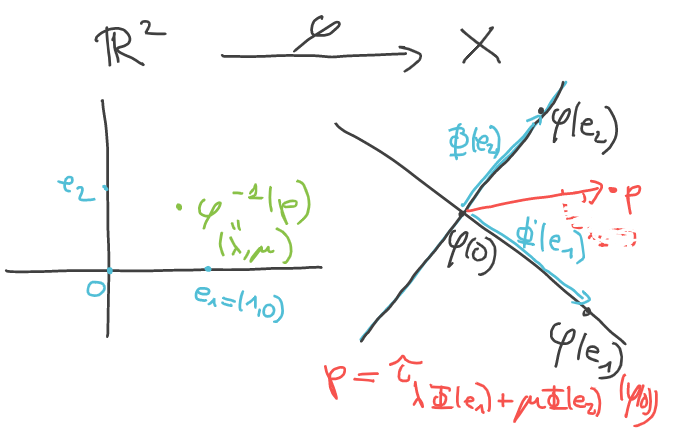
\includegraphics[width=0.7\linewidth]{figures/affine_koordinatenabbildung_r_2}
        \label{fig:affine_koordinatenabbildung_r_2}
    \end{figure}
\end{definition*}
\section{Das Teilverhältnis}
\begin{idee*}
    Seien 3 Punkte \( p_0,p_1,p \) auf einer Gerade \( l \) (\zb im \( \reals^3 \)) gegeben, \( p_0\neq p_1 \).
    \begin{figure}[H]
        \centering
        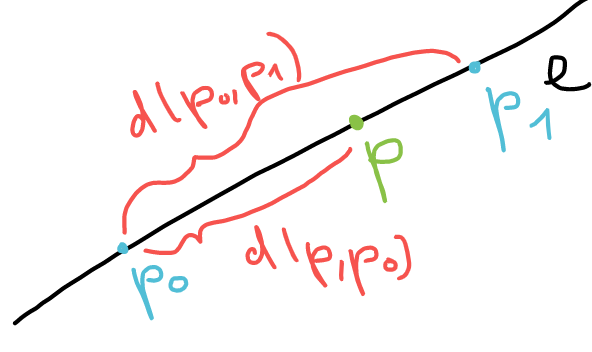
\includegraphics[width=0.5\linewidth]{figures/gerade_teilverhaeltnis}
        \caption*{}
        \label{fig:gerade_teilverhaeltnis}
    \end{figure}
    Sei \( \lambda=\frac{d(p,p_0)}{d(p_1,p_0)} \), mit \( d \) dem euklidischen Abstand, dann können wir die Lage von \( p \) auf \( l \) durch \( \lambda \) (und der Information, ob \( p \) \enquote{rechts oder links} von \( p \) liegt) bestimmen.
\end{idee*}
\begin{definition*}
    Sei \( X \) ein affiner Raum über \( K \), \( Y\subseteq X \) eine affine Gerade, \( p_0,p_1,p\in Y \) und \( p_0\neq p_1 \). Dann nennen wir das eindeutig bestimmte Element \( \lambda\in K \) mit \( \vv{p_0 p}=\lambda \vv{p_0 p_1} \) das Teilverhältnis von \( p_0,p_1,p \). Schreibe \( \lambda=\teilverhaeltnis(p_0,p_1,p) \). In \( \characteristic(K)\neq 2 \) nennen wir \( p \) Mittelpunkt von \( p_0,p_2 \) wenn \( \teilverhaeltnis(p_0,p_1,p)=\frac{1}{2} \).
\end{definition*}
\begin{bemerkungen*}
    \begin{enumerate}
        \item Es gilt \( T(Y)=K\vv{p_0p_1} \). Damit ist \( \lambda \) wohldefiniert und existiert.
        \item \( p_0,p_1 \) ist eine affine Basis von \( Y \). Damit existiert ein Koordinatensystem
        \begin{align*}
            \phi\maps K\to Y,\logicspace \begin{aligned}[t]
                \phi(0)&=p_0\\
                \phi(1)&=p_1
            \end{aligned}
        \end{align*}
        und es gilt \( \teilverhaeltnis(p_0,p_1,p)=\inv{\phi(p)} \).
    \end{enumerate}
    
\end{bemerkungen*}
\begin{frage*}
    Wie verhält sich das Teilverhältnis unter affinen Abbildungen?
    \begin{figure}[H]
        \centering
        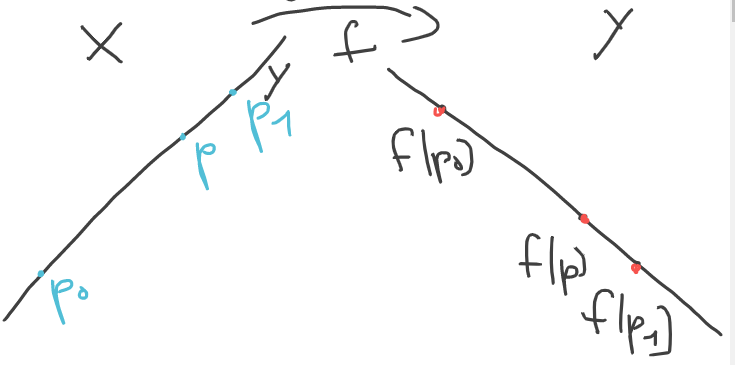
\includegraphics[width=0.7\linewidth]{figures/affine_abbildungen_wirkung_auf_teilverhaeltnis}
        \label{fig:affine_abbildungen_wirkung_auf_teilverhaeltnis}
    \end{figure}
    
\end{frage*}